\chapter{Aufgabe 1}

\section{Teil 1)}

\textit{Um welchen Bus handelt es sich hier? Begründen Sie Ihre Antwort.}\\


\noindent
In Abbildung~\ref{fig:bus} (1) ist ein \textbf{I$^2$C-Bus} dargestellt.
Die einzelnen Geräte sind über eine \texttt{SCL}\footnote{\textit{Serial Clock Line}}- und eine \texttt{SDA}\footnote{Serial Data Line}-Leitung mit dem Bus verbunden (vgl.~\cite[168]{ES4}). Diese zwei Leitungen sind charakteristisch für das I$^2$C-Bus-System.\\
Die Selektion eines Gerätes erfolgt hierbei über die jeweilige Busadresse (vgl.~\cite[170]{ES4}).


\begin{figure}
    \centering
    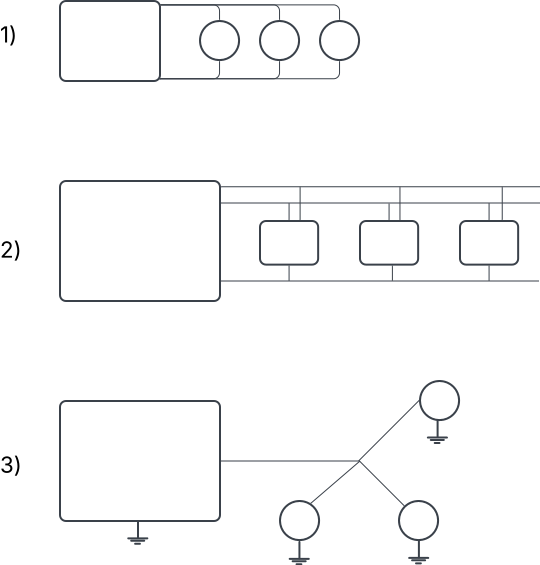
\includegraphics[scale=0.3]{aufgabe 1/img/bus.svg}
    \caption{Skizze der in Aufgabe 1 vorgestellten Bus-Systeme. (Quelle: in Anlehnung an Abbildung 1, 2, 3 aus Aufgabe 1, Einsendeaufgaben 5)}
    \label{fig:bus}
\end{figure}


\section{Teil 2)}

\textit{Um welchen Bus handelt es sich hier? Begründen Sie Ihre Antwort.}\\

\noindent
In Abbildung~\ref{fig:bus} 2) ist ein SPI-Bus dargestellt: Auch wenn mehrere Leitungen charakteristisch für einen SPI-Bus sind (\texttt{CS}, \texttt{SCLK}, \texttt{SDO}, \texttt{SDI},vgl.~\cite[179]{ES4}), könnte es sich bei den dargestellten Leitungen handeln um:
\begin{itemize}
    \itemsep0.5em
    \item \texttt{CS} zur Auswahl des \textit{Slaves}
    \item \texttt{SDO} (\textit{Serial Data Output}) zum Senden
    \item \texttt{SDI} (\textit{Serial Data Input}) zum Empfangen
\end{itemize}


\section{Teil 3)}

\textit{Um welchen Bus handelt es sich hier? Begründen Sie Ihre Antwort.}\\

\noindent
In Abbildung~\ref{fig:bus} (3) ist ein \textbf{1-Wire-Bus} dargestellt.
Der Bus verfügt über einen \texttt{GND}-Anschluss, die verschiedenen Devices sind über \textit{genau eine} Leitung mit der Bus-Komponente verbunden und verfügen selber über einen Masse-Anschluss (\texttt{GND}).
Die Stromversorgung und die Datenübertragung erfolgt - dem Namen entsprechend - über \textit{eine} Verbindung\footnote{
\url{https://www.analog.com/en/resources/technical-articles/guide-to-1wire-communication.html}, abgerufen 17.04.2025
}.

\section{Teil 4)}

\textit{Gibt es einen Unterschied zwischen I$^2$C-Bus und SMB-Bus?}\\

\noindent
Wie \textit{Bollenbacher} in~\cite[92]{ES5} erläutert, können beide Bussysteme grundsätzlich ``als kompatibel betrachtet werden``.
Die Unterschiede liegen im Detail auf elektrischer Ebene:

\blockquote[]{
    ``Die Übertragung der Signale über den \texttt{SMB}-Bus entspricht der über den
    I$^2$C-Bus. Unterschiede betffen die Pegel einiger elektrischer Signale, Geschwindigkeiten und den Leistungsverbrauch der Chips.``
}